% vim: set textwidth=78 autoindent:

\section{Using QGIS Core Plugins}\label{sec:core_plugins}\index{plugins!core}

% when the revision of a section has been finalized, 
% comment out the following line:
\updatedisclaimer

QGIS currently contains 16 core plugins that can be loaded using the Plugin Manager.
Table \ref{tab:core_plugins} lists each of the core plugins along with a description of 
their purpose and the toolbar-icon.

% minipage is needed to appear the footnote under the table
% SH
\begin{minipage}{\textwidth}
\begin{table}[H]
\centering
\caption{QGIS Core Plugins}\label{tab:core_plugins}\medskip
\small
 \begin{tabular}{|l|l|p{4in}|}
\hline \textbf{Icon} & \textbf{Plugin} & \textbf{Description}\\
\hline

\includegraphics[width=0.7cm]{delimited_text}
 & Add Delimited Text Layer \index{plugins!delimited text} & Loads and displays delimited text files containing x,y coordinates\\
\hline

\includegraphics[width=0.7cm]{coordinate_capture}
 & Coordinate Capture \index{plugins!coordinate capture}& Capture mouse coordinate in different CRS\\
\hline 

\includegraphics[width=0.7cm]{copyright_label}
 & Copyright Label \index{plugins!copyright}& Draws a copyright label with information\\
\hline 

\includegraphics[width=0.7cm]{dxf2shp_converter}
 & DXF2Shape Converter \index{plugins!DXF2Shape}& Converts from DXF to SHP file format\\
\hline

\includegraphics[width=0.7cm]{gps_importer}
 & GPS Tools \index{plugins!gps}& Tools for loading and importing GPS data\\
\hline

\includegraphics[width=0.7cm]{grass}
 & GRASS \index{plugin!grass toolbox} & Activates the mighty GRASS Toolbox\\
\hline

\includegraphics[width=0.7cm]{georeferencer}
 & Georeferencer \index{plugin!georeferencer} & Adding projection info to Rasterfiles\\
\hline

\includegraphics[width=0.7cm]{grid_maker}
 & Graticule Creator \index{plugins!graticule}& Create a latitude/longitude grid and save as a shapefile\\
\hline

\includegraphics[width=0.7cm]{interpolation}
& Interpolation plugin \index{plugins!Interpolation}& Interpolation on base of vertices of a vector layer\\
\hline

\includegraphics[width=0.7cm]{mapserver_export}
& MapServer Export Plugin \index{plugins!MapServer Export}& Export a saved QGIS project file to a MapServer map file \\
\hline

\includegraphics[width=0.7cm]{north_arrow}
& North Arrow \index{plugins!north arrow}& Displays a north arrow overlayed onto the map\\
\hline

\includegraphics[width=0.7cm]{ogr_converter}
 & OGR Layer Converter \index{plugins!OGR converter} & Translate vector layers between formats supported by OGR-Library\\
\hline
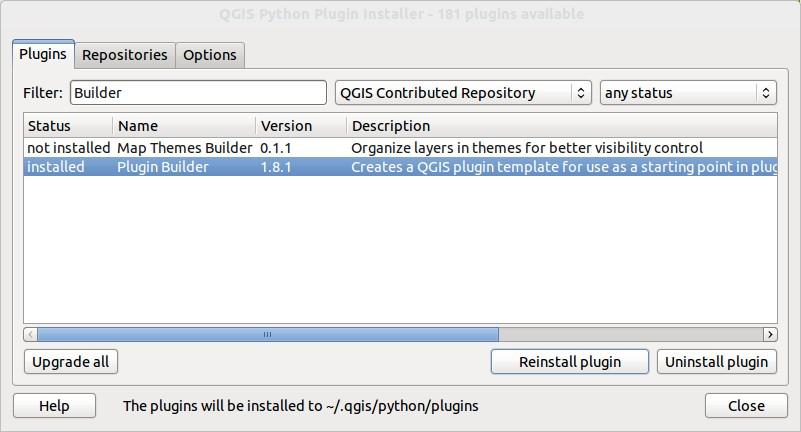
\includegraphics[width=0.7cm]{plugin_installer}
 & Plugin Installer \index{plugins!Plugin Installer} & Downloads and installs QGIS python plugins\\
\hline

\includegraphics[width=0.7cm]{icon_buffer}
 & SPIT \index{plugins!spit}& Shapefile to PostgreSQL/PostGIS Import Tool \\
\hline

\includegraphics[width=0.7cm]{scale_bar}
 & Scalebar \index{plugins!scalebar}& Draws a scale bar\\
\hline

\includegraphics[width=0.7cm]{mIconAddWfsLayer}
 & WFS & Load and display WFS layer \\
\hline
\end{tabular}
\end{table}
\end{minipage}

\normalsize

\begin{Tip}\caption{\textsc{Plugins Settings Saved to Project}}\index{plugins settings}
\qgistip{When you save a .qgs project, any changes you have made to NorthArrow, ScaleBar and Copyright plugins will be saved in the project and restored next time you load the project.}
\end{Tip}
